%; whizzy chapter
% -initex iniptex -latex platex -format platex -bibtex jbibtex -fmt fmt
% 以上 whizzytex を使用する場合の設定。

%     Kansai Debian Meeting resources
%     Copyright (C) 2007 Takaya Yamashita
%     Thank you for Tokyo Debian Meeting resources

%     This program is free software; you can redistribute it and/or modify
%     it under the terms of the GNU General Public License as published by
%     the Free Software Foundation; either version 2 of the License, or
%     (at your option) any later version.

%     This program is distributed in the hope that it will be useful,
%     but WITHOUT ANY WARRANTY; without even the implied warranty of
%     MERCHANTABILITY or FITNESS FOR A PARTICULAR PURPOSE.  See the
%     GNU General Public License for more details.

%     You should have received a copy of the GNU General Public License
%     along with this program; if not, write to the Free Software
%     Foundation, Inc., 51 Franklin St, Fifth Floor, Boston, MA  02110-1301 USA

%  preview (shell-command (concat "evince " (replace-regexp-in-string "tex$" "pdf"(buffer-file-name)) "&"))
% 画像ファイルを処理するためにはebbを利用してboundingboxを作成。
%(shell-command "cd image200708; ebb *.png")

%%ここからヘッダ開始。

\documentclass[mingoth,a4paper]{jsarticle}
\usepackage{kansaimonthlyreport}
\usepackage[dvips]{xy}
\usepackage{ulem}

% 日付を定義する、毎月変わります。
\newcommand{\debmtgyear}{2013}
\newcommand{\debmtgdate}{24}
\newcommand{\debmtgmonth}{2}
\newcommand{\debmtgnumber}{69}

\begin{document}

\begin{titlepage}

% 毎月変更する部分、本文の末尾も修正することをわすれずに

 第\debmtgnumber{}回 関西 Debian 勉強会資料

\vspace{2cm}

\begin{center}
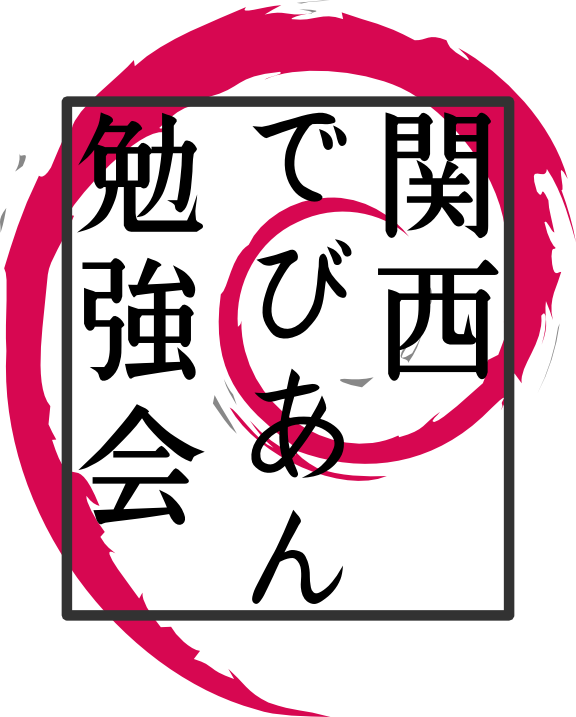
\includegraphics{image200802/kansaidebianlogo.png}
\end{center}

\begin{flushright}
\hfill{}関西 Debian 勉強会担当者 佐々木・倉敷・のがた・かわだ \\
\hfill{}\debmtgyear{}年\debmtgmonth{}月\debmtgdate{}日
\end{flushright}

\thispagestyle{empty}
\end{titlepage}

\dancersection{Introduction}{Debian JP}

\vspace{1em}

 関西Debian勉強会はDebian GNU/Linuxのさまざまなトピック
 (新しいパッケージ、Debian特有の機能の仕組、Debian界隈で起こった出来事、
 などなど)について話し合う会です。

 目的として次の三つを考えています。
 \begin{itemize}
  \item MLや掲示板ではなく、直接顔を合わせる事での情報交換の促進
  \item 定期的に集まれる場所
  \item 資料の作成
 \end{itemize}

 それでは、楽しい一時をお楽しみ下さい。

\newpage

\begin{minipage}[b]{0.2\hsize}
 {\rotatebox{90}{\fontsize{80}{80}
{\gt 関西 Debian 勉強会}}}
\end{minipage}
\begin{minipage}[b]{0.8\hsize}
\hrule
\vspace{2mm}
\hrule
\setcounter{tocdepth}{1}
\tableofcontents
\vspace{2mm}
\hrule
\end{minipage}

\dancersection{最近のDebian関係のイベント報告}{Debian JP}

\subsection{第 68 回関西 Debian 勉強会}

68 回目の関西 Debian 勉強会は 1 月 27 日(日)に国際奈良学セミナーハウス
研修施設で行なわれました。

紀野さんの「Using Drupal on Debian」は、Drupal と Debian のお作法の違い
がよくみえるよいセッションでした。

野方さんの「月刊 Debian Policy オペレーティングシステム」は一回で収まら
ない内容だったので前半のユーザとグループまでとなりました。init スクリプ
ト以降は次回となりましたので続きが楽しみです。

初の奈良開催でしたが、会場は奈良公園内近くの雰囲気のよい場所でした。今
年は大阪以外の場所でも勉強会を開催したいですね。


\subsection{第 97 回東京エリア Debian 勉強会 2013年2月勉強会 2013 OSC出張}

97 回目の東京エリア Debian 勉強会は 2 月 23 日(土)にオープンソースカン
ファレンス 2013 Tokyo/Spring にて出張版として開催されました。

セミナーでは野島さんによる「Debian update - Debianの最新動向について語
ります」の発表が行なわれました。

\subsection{オープンソースカンファレンス 2013 Hamamatsu}
2 月 9 日(土)に浜松市市民協働センターで開催されたオープンソースカンファ
レンス 2013 Hamamatsu に東京エリア  Debian 勉強会でブース出展しました。

\subsection{第 1 回 Debian パッケージング道場}
2 月 9 日(土)に京都大学で第 1 回目の Debian パッケージング道場が開催さ
れました。

当日は 9 名の参加者が午前中に岩松さんから基本的なパッケージの作成方法と
最新のパッケージング事情と使い方の説明をうけ、午後から各自が思い思いの
パッケージ作成を行ないました。

TitanPad に資料がまとめられていますので参照してみてください。
\url{http://debian-pkg-dojo.titanpad.com/1}

\dancersection{事前課題}{Debian JP}

今回は以下の課題を出題しました.
\begin{screen}
  \begin{enumerate}
  \item リリースノートの「付録 B. preseed を利用したインストールの自動化」\footnote{\url{http://www.debian.org/releases/stable/i386/apb.html.ja}}を読んできて下さい。

    また、読んで気になる点などがあれば、教えて下さい。
  \item Wheezy もしくは sid 環境に apt-get install ruby してきて下さい。
  \item 普段(業務もしくは趣味等)お使いの Ruby ソフトウェアがあれば、教えて下さい。

    また、それが Debian パッケージになっていないならば、ご指摘下さい。
  \end{enumerate}
\end{screen}

参加者の皆さんの解答は以下の通りです。

\begin{prework}{ 西山和広 }
  \begin{enumerate}
  \item ちゃんと読んでいたら長くなってしまったので \url{https://gist.github.com/znz/831f7bd6b0c5eff06530} に置きました。

    \begin{itemize}
    \item[B.1.1.]
      hd-media の hd が何なのか気になりました。
    \item[B.2.1.]
      インストーラが確実に正しい事前設定ファイルを取得するのに、このファイルのチェックサムを指定できます。現在、これには md5sum 値の指定が必要です。指定した値と事前設定ファイルの値は一致し
      なければなりません。一致しない場合は、インストーラは事前設定ファイルを使用しません。
   
      必須かどうかわかりにくいと思いました。
    \item[B.2.2.]
      注意

      現在の Linux カーネル (2.6.9 以降) では、最大 (インストーラがデフォルトで指定するオプションを含め) コマンドラインオプションを 32 個、環境オプションを 32 個受け取れます。この数を超え    ると、カーネルはパニック (クラッシュ) してしまいます (以前のカーネルではこの数字がもっと少ないです)。
   
      長さの制限があるのかどうか気になりました。

    \item[B.2.3.]
    auto ブートラベルは、まだどこにも定義されていません。
   
    「auto url=...」というのが使えるのかどうかわかりませんでした。

    \item[B.2.5.]
    この文字列で、ネットワーク上の全マシンに preseed でインストールするのではなく、特定のホストに対して行うようにもできます。
   
    この文字列とは?

    \item[B3]
    型と値の間はよくありません。
   
    型はタイプ (質問タイプ) でしょうか?

    \item[B.4.1. 地域化]
    この方法は費用に使うのが容易ですが、言語、国、ロケールの利用可能な組み合わせをすべて preseed できるわけではありません[29]。言語と国は、どちらもブートパラメータで指定できます。
   
    費用に使うのが容易というところの意味が分かりませんでした。

    \item[B.4.5.]
    パスワードを知っている事前設定ファイルが誰でもアクセスできるために、
   
    「事前設定ファイルが」は「事前設定ファイルは」とか「事前設定ファイルを」とかの方が良いのではないでしょうか。

    \item[B.4.10.]
    このパラメータの値は、カーネルコマンドラインにそのまま渡されるので、カンマか空白で区切ったパッケージのリストを取れます。
   
    カーネルコマンドラインでは値に空白区切りは使えないはずなので、誤訳のように見えます。

    \item[B.5.2.]
    この場合でも質問は行われます。
   
    ここも誤訳でしょうか? 英語の方は「質問済み状態のまま」(だから質問されない) (ので後続の文で未質問状態に戻す、と続く) という意味に見えます。

    \item[B.5.2.]
    派ケージ
   
    typo?

    \item[B.5.3.]
    他のファイルでより確かな設定を指定する
   
    specific を「確かな」と訳すのはちょっと違うように感じました。

  \end{itemize}

  \item インストールしました。
  \item nadoka という IRC の proxy のようなものを使っているのですが、新しいバージョンが Debian パッケージになっていません。
  \end{enumerate}
\end{prework}

\begin{prework}{ かわだてつたろう }
  \begin{enumerate}
  \item 読んでみました。

    preseed を使ったことはないのですが、警告があるようにパーティション分割がはまりそうな気がします。
  \item してあります。
  \item redmine, nokogiri, rabbit
  \end{enumerate}
\end{prework}

\begin{prework}{ 山城の国の住人 久保博 }
  \begin{enumerate}
  \item はい、今から頑張ります。
  \item はい。schroot の中に作った sid 環境にインストールしておきます。
  \item Redmine を使っています。
  \end{enumerate}
\end{prework}

\begin{prework}{ murase\_{}syuka }
  \begin{enumerate}
  \item 軽く読んでみたが良く分からない
  \item rvmでinstall済み
  \item rvm/irb(pry)/rails
  \end{enumerate}
\end{prework}

\begin{prework}{ のがたじゅん }
  \begin{enumerate}
  \item はい読みました。が、いまだにHDDのパーティションの切り方がよくわかってなかったり。

    \url{http://www.nofuture.tv/linux/debianautoinstall}
  \item はい。入ってます。
  \item tDiaryを使ってます
  \end{enumerate}
\end{prework}

\begin{prework}{ よしだともひろ }
  \begin{enumerate}
  \item 読んでおきます。
  \item sid環境で、apt-get install ruby 実行しました。
  \item rabbitくらいかも。
  \end{enumerate}
\end{prework}

\begin{prework}{ yyatsuo }
  \begin{enumerate}
  \item 一通り読んでみました
  \item Ruby 1.9.1 インストール済みです
  \item 普段使うのは RedMine

    今までに使ったことがあるのは Milkode と Termtter
  \end{enumerate}
\end{prework}

\begin{prework}{ 佐藤誠 }
  \begin{enumerate}
  \item 今読んでます。

    ちょっと試してみたいけど、時間が...(汗
  \item 仮想環境のsqueezeを、昨晩ようやくwheezyにあげました。

    えーと、ruby も入ってるはず(未確認)
  \item tdiaryでブログを書いています。
  \end{enumerate}
\end{prework}

\begin{prework}{ 佐々木洋平 }
  \begin{enumerate}
  \item preceed よく使ってます
  \item 普段から使ってます。そろそろ mruby と ruby2.0 を入れたいですね。
  \item redmine と Jekyll がないと途方にくれます。あと、今回のプレゼンは rabbit です。
  \end{enumerate}
\end{prework}

\begin{prework}{ 大林 }
  \begin{enumerate}
  \item 一通り読みました。
  \item Wheezyの実験用環境にインストールしました。

    ただネットワークの向こう側のVMの上なので、会場では使えないかもしれません。

    会場でネットワークがもし使えればいけるのですが。
  \item yard, rmagick, test-unit, NArray, depq など
  \end{enumerate}
\end{prework}

\begin{prework}{ kazuhito.sumpic }
(無回答)
\end{prework}

\dancersection{Debian Installer トラブルシューティング}{Yuryu}

\subsection{自己紹介}
\begin{itemize}
\item Yuryu (twitter: @Yuryu)
\item 某社でインフラエンジニアしてます
\item potato → woody → (浮気) → Ubuntu(Gusty) → ... → Ubuntu(Precise)
\item 会社では Debian 使ってます
\item 好きなコマンドは xargs
\end{itemize}

\subsection{Preseed}
\subsubsection{Preseed とは}
\begin{itemize}
\item Debian Installer の応答ファイル
\item すべての選択肢が選べる
\item PXE と組み合わせると強い
  \begin{itemize}
  \item 単体でも使えます(少々面倒)
  \end{itemize}
\end{itemize}

\begin{commandline}
locale=en_US language=en country=JP
console-keymaps-at/keymap=jp106
keyboard-configuration/xkb-keymap=jp106
interface=eth0 hostname=debian
domain=local url=http://holo.yuryu.jp/preseed.cfg
DEBCONF_DEBUG=5
\end{commandline}

\subsubsection{bootオプションの必要性}
\begin{itemize}
\item Preseed ファイルが読まれるのは、ネットワークの設定が終わってから
\item ネットワーク設定前にもインストーラーの質問はある
\item →ブートオプションとして渡す
\item 長いので手打ちは無理、PXE を使う
\end{itemize}

\subsubsection{expert install}
\begin{itemize}
\item expert options → automated install
\item 途中で preseed ファイルを指定できる
\item とりあえず試すにはこっち
\end{itemize}

\subsubsection{url}
\begin{itemize}
\item preseed ファイルの場所
\item http, ftp, tftp で指定
\item https は使えない(!)
\end{itemize}

\subsubsection{ファイルの中身}
\begin{itemize}
\item 「d-i 項目名 指定」の羅列
\end{itemize}

\begin{commandline}
### Clock and time zone setup
# Controls whether or not the hardware clock is set to UTC.
d-i clock-setup/utc boolean true

# You may set this to any valid setting for $TZ; see the contents of
# /usr/share/zoneinfo/ for valid values.
d-i time/zone string Asia/Tokyo

# Controls whether to use NTP to set the clock during the install
d-i clock-setup/ntp boolean true
# NTP server to use. The default is almost always fine here.
d-i clock-setup/ntp-server string ntp.nict.go.jp
\end{commandline}
%$

\subsubsection{ファイルの書き方}
\begin{itemize}
\item 基本的にはサンプル通り
\item でも、いくつか落とし穴が...
  \begin{itemize}
  \item 一番大変なのが partitioning
  \end{itemize}
\end{itemize}

\subsection{partitioning}

\subsubsection{partitioning}
\begin{itemize}
\item d-i partman-auto/choose\_recipe
  \begin{itemize}
  \item atomic - / 一発
  \item home - /home だけ分ける
  \item multi - /home, /usr, /var, /tmp
  \end{itemize}
\item d-i partman-auto/expert\_recipe
\end{itemize}

\subsubsection{recipe}
\begin{commandline}
d-i partman-auto/expert_recipe string                         \
      boot-root ::                                            \
              40 50 100 ext2                                  \
                      $primary{ } $bootable{ }                \
                      method{ format } format{ }              \
                      use_filesystem{ } filesystem{ ext2 }    \
                      mountpoint{ /boot }                     \
              .                                               \
              500 10000 -1 ext4                               \
                      method{ format } format{ }              \
                      use_filesystem{ } filesystem{ ext4 }    \
                      mountpoint{ / }                         \
              .                                               \
              64 512 300% linux-swap                          \
                      method{ swap } format{ }                \
              .
\end{commandline}

\clearpage

\subsubsection{レシピ形式}

レシピ名 ::

\ 最低容量(MB) 優先度 最大容量 FS

\ パーティション内容 .

\begin{commandline}
 500 1000 -1 ext4 \
 method{ format } format{ } \
 use_filesystem{ } filesystem{ ext4 } \
 mountpoint{ /home }
\end{commandline}

\subsubsection{容量}
\begin{itemize}
\item 最大を -1 にすると空き容量をすべて使う
\item 優先度は数字が大きなほうが低い
\item 最小=最大にせず100MB程度の幅をもたせる
\end{itemize}

\subsubsection{method}
\begin{itemize}
\item format
  \begin{itemize}
  \item 通常通りフォーマットして使用
  \end{itemize}
\item swap
  \begin{itemize}
  \item スワップパーティションとして使用
  \end{itemize}
\item keep
  \begin{itemize}
  \item 何もせず区画だけ作る
  \end{itemize}
\end{itemize}

\subsubsection{ファイルシステム}
\begin{itemize}
\item 容量の右側に書くものと、filesystem\{ \}
\item 基本的には同じ
\item ext[2-4], xfs, btrfs, jfs, linux-swap
\item keep のときは無視される(free でもok)
\end{itemize}

\subsubsection{お約束}
\begin{itemize}
\item 冗長に見えても、省略できないもの
\item format\{ \}
\item use\_filesystem\{ \}
\item filesystem\{ ext4 \}
\end{itemize}

\subsection{ハマりました}

\subsubsection{primary}
\begin{itemize}
\item \$primary\{ \} プライマリ必須指定
\item \$logical\{ \} もありそう?
  \begin{itemize}
  \item 実は無い
  \item 省略すると logical になる
  \end{itemize}
\end{itemize}

\subsubsection{一行で書く}
\begin{itemize}
\item 行末に \textbackslash を書いて、一行につなげて書く
\item \textbackslash の後にスペースがあるとそこで切れます
\end{itemize}
 
\subsubsection{レシピ名}
\begin{itemize}
\item レシピ名が必須
\item partman-auto/choose\_recipe とは無関係
  \begin{itemize}
  \item expert recipe 使うなら書いてはいけない
  \end{itemize}
\item 何を書いても動作に関係なし...
\end{itemize}

\begin{commandline}
d-i partman-auto/expert_recipe string                         \
      boot-root ::                                            \
\end{commandline}

\subsubsection{スペースの扱い}
\begin{itemize}
\item 基本的にはスペース必須
\item 開きカッコの手前はスペース不可
  \begin{itemize}
  \item ○ method\{\_format\_\}
  \item × method\_\{\_format\_\}
  \end{itemize}
\item grep でパースしてるので厳格です...
\end{itemize}

\subsubsection{レシピ、認識されてる?}
\begin{itemize}
\item /tmp/expert\_recipe
\item 実際に使われたレシピが入る
\end{itemize}

\begin{commandline}
~ # cd /tmp
/tmp # ls
connection_type  expert_recipe    mdadm.conf
/tmp # cat expert_recipe
boot-root :: 40 50 100 ext3 #primary{ } $bootable{ } method{ format } format{ } use_filesystem{ } filesystem{ ext3 }
mountpoint{ /boot } . 500 10000 1000000000 ext3 method{ format } format{ } use_filesystem{ } filesystem{ ext3 }
mountpoint{ / } . 64 512 300% linux-swap method{ swap } format{ } .
/tmp #
\end{commandline}
%$

\subsubsection{その他条件文}
\begin{itemize}
\item \$iflabel\{ label \} - ラベルが一致
\item \$defaultignore\{ \} - LVM を使わない時無視
\item \$lvmok\{ \} - LVM にしても良い
\item \$lvmignore\{ \} - LVM の場合は無視
\end{itemize}

\subsubsection{パーティション再利用}
\begin{itemize}
\item 既存のパーティションを再利用
\item \$reusemethod\{ \}
  \begin{itemize}
  \item method(format, swap) が同一なら再利用
  \item 主に biosgrub, swap 向け?
  \end{itemize}
\item \$iflabel\{ label \} と組み合わせる
\item \url{http://lists.debian.org/debian-boot/2011/04/msg00333.html}
\end{itemize}

\subsection{その他troubleshoot}
\subsubsection{d-i じゃない行もある}
\begin{itemize}
\item d-i で始まらない行もある
  \begin{itemize}
  \item tasksel
  \item popularity-contest
  \end{itemize}
\item コピペ事故に注意
\end{itemize}

\subsubsection{止まったら}
\begin{itemize}
\item syslog を確認
\item INPUT ... の行がパラメーター名
\end{itemize}

\subsubsection{ログ}
\begin{itemize}
\item Alt+F4 のログ
\item インストール中 /var/log/syslog
\item インストール後 /var/log/installer/syslog
\item DEBCONF\_DEBUG が必須
\end{itemize}

\subsubsection{こわくないよ}
\begin{itemize}
\item debian installer の実態はシェルスクリプト
\item 各ディレクトリを for で順に呼んでる
\item 項目名で grep してみるとヒントが
\end{itemize}

\subsubsection{debian/*.templates}
\begin{itemize}
\item debian-installer の各種パッケージの debian/*.templates
\item 変数名、型、説明が揃ってる
\item リファレンス代わりになります
\end{itemize}

\begin{commandline}
Template: partman-partitioning/bootable_logical
Type: boolean
Default: false
# :sl2:
_Description: Are you sure you want a bootable logical partition?
 You are trying to set the bootable flag on a logical partition. The
\end{commandline}

\subsubsection{debconf-get-selections}
\begin{itemize}
\item インストール済みOSから設定を取得
\item debconf-get-selections --installer
\item デフォルト値も含めて大量に出る
  \begin{itemize}
  \item 必要な物を取捨選択する必要あり
  \end{itemize}
\end{itemize}

\subsubsection{Ubuntu 対応}
\begin{itemize}
\item 基本的には同じ
\item いくつか追加の質問
  \begin{itemize}
  \item d-i pkgsel/update-policy select none
  \item d-i user-setup/allow-password-weak boolean true
  \item d-i user-setup/encrypt-home boolean false
  \end{itemize}
\item 詳しくは \url{https://help.ubuntu.com/lts/installation-guide/i386/preseed-contents.html}
\end{itemize}

\subsection{まとめ}
\begin{itemize}
\item 困ったら syslog を観る
\item recipe はスペースに気をつける
\item DEBCONF\_DEBUG=5 重要!
\end{itemize}

\clearpage

\dancersection{Ruby In Wheezy}{佐々木洋平}

\vspace{1em}

次期安定版 Debian 7.0 (Wheezy) における Ruby 環境について、%
特に複数の Ruby 実装の共存と Gem とのお付き合いの仕方について、
簡単にお話しします。

\subsection{``Ruby'' in Wheezy}

Ruby には複数の実装が存在しています。
Debian Wheezy では以下の Ruby インタープリタが使用できます:
\begin{table}[h!]
  \centering
  \begin{tabular}{lll}
    インタープリタ & パッケージ名       & 注意書き \\
    MRI 1.8.7      & \texttt{ruby1.8}   &          \\
    MRI 1.9.3      & \texttt{ruby1.9.3} & \texttt{ruby1.9.1} パッケージの実態は \texttt{ruby1.9.3} だったりします。 \\
    JRuby          & \texttt{jruby}     & パッケージは Debian Java Maintainers によって管理されています \\
    Rubinius       & \texttt{rubinius}  & 現在作業中です. ITP\#591817 \\
    mruby          & \texttt{mruby}     & 現在作業中です. ITP\#697835 \\
  \end{tabular}
\end{table}
%
\newline
「\texttt{ruby1.9.1} パッケージの実態は \texttt{ruby1.9.3} だったりします。」について、
Ruby の soname が変わっていないので \texttt{libruby1.9.1} 等のパッケージが残っており、
\texttt{ruby1.9.3} パッケージは \texttt{/usr/bin/ruby1.9.1} への
symbolic link を提供するだけだったりします。
\begin{commandline}
% dpkg -S ruby1.9.3
ruby1.9.3: /usr/bin/ruby1.9.3
ruby1.9.3: /usr/share/man/man1/ruby1.9.3.1.gz
ruby1.9.3: /usr/share/doc/ruby1.9.3
ruby1.9.3: /usr/share/doc/ruby1.9.3/NEWS.Debian.gz
ruby1.9.3: /usr/share/doc/ruby1.9.3/NEWS.gz
ruby1.9.3: /usr/share/doc/ruby1.9.3/changelog.Debian.gz
ruby1.9.3: /usr/share/doc/ruby1.9.3/changelog.gz
ruby1.9.3: /usr/share/doc/ruby1.9.3/copyright
ruby1.9.3: /usr/share/doc/ruby1.9.3/README.gz
% ls -la /usr/bin/ruby1.9.3
lrwxrwxrwx 1 root root 9 Feb 23 23:44 /usr/bin/ruby1.9.3 -> ruby1.9.1*
\end{commandline}
他にも、\texttt{Topaz} や \texttt{HPC Ruby Compiler} など、(個人的に)気になる実装がありますが、まだ Debian でどうこうというお話にはなっていません。

\subsection{複数の Ruby 実装の切り替え}

さて、これだけ複数の Ruby 実装があると、それを切り替えて使いたくなるのが人情だと思います。
Debian には、同じ機能を提供するソフトウェアをきりかえる \texttt{update-alternatives} という仕組みが既にあります。
ですが、\texttt{/usr/bin/ruby} を切り替えたら \texttt{gem} や \texttt{irb} なんかも切り替えたくなるでしょう。
そのため、これらを一度に変換するためのコマンドが提供されています。

\subsubsection{システム全体でデフォルトの Ruby を切り替えるには?: \texttt{ruby-switch}}

システム全体でデフォルトの Ruby インタープリタを選択するために、ruby-switch パッケージが使用可能です。 これは root として(もしくは sudo を使って)実行する必要があります。
\begin{commandline}
# ruby -v
ruby 1.8.7 (2011-06-30 patchlevel 352) [x86_64-linux]
# ruby-switch --list
ruby1.8
ruby1.9.1
# ruby-switch --set ruby1.9.1
update-alternatives: using /usr/bin/gem1.9.1 to provide /usr/bin/gem (gem) in manual mode.
update-alternatives: using /usr/bin/ruby1.9.1 to provide /usr/bin/ruby (ruby) in manual mode.
# ruby -v
ruby 1.9.3p0 (2011-10-30 revision 33570) [x86_64-linux]
# ruby-switch --auto
update-alternatives: using /usr/bin/ruby1.8 to provide /usr/bin/ruby (ruby) in auto mode.
update-alternatives: using /usr/bin/gem1.8 to provide /usr/bin/gem (gem) in auto mode.
# ruby -v
ruby 1.8.7 (2011-06-30 patchlevel 352) [x86_64-linux]
\end{commandline}

\subsubsection{ユーザ毎にデフォルトの Ruby インタープリタを選択するには: \texttt{rbenv}}

ユーザアカウント毎にデフォルトの Ruby インタープリタを切り替えるには、rbenv パッケージを使うのが良いでしょう。
\begin{commandline}
% ruby -v
ruby 1.8.7 (2011-06-30 patchlevel 352) [x86_64-linux]
% rbenv init
# Load rbenv automatically by adding
# the following to ~/.bash_profile:

eval ``$(rbenv init -)"
% echo 'eval ``$(rbenv init -)"' >> ~/.bash_profile # or ~/.bashrc, depends on your setup
% rbenv versions
% rbenv alternatives
% rbenv versions
  1.8.7-debian
  1.9.3-debian
% rbenv global 1.9.3-debian
% ruby -v
ruby 1.8.7 (2011-06-30 patchlevel 352) [x86_64-linux]
\end{commandline}
%%$
一見ちゃんと動作していないように見えますが、これは現在実行中のシェルが "ruby" の位置として /usr/bin/ruby をキャッシュしているからです。新しいシェルを開始した後には、デフォルトの Ruby を行ったり来たり切り替えることができます。
\begin{commandline}
% ruby -v
ruby 1.8.7 (2011-06-30 patchlevel 352) [x86_64-linux]
% rbenv global 1.9.3-debian
% ruby -v
ruby 1.9.3p0 (2011-10-30 revision 33570) [x86_64-linux]
% rbenv global 1.8.7-debian
% ruby -v
ruby 1.8.7 (2011-06-30 patchlevel 352) [x86_64-linux]
\end{commandline}

\subsubsection{Debian パッケージになっていない Ruby をインストールするには: \texttt{ruby-build}}

\texttt{ruby-build} を使用することで、Debian でまだ使用可能になっていない Ruby インタープリタをインストールすることができます。
しかしながら、このパッケージの README.Debian ファイルに書かれている内容に注意して下さい:
\begin{commandline}
  While ruby-build is a great tool to build Ruby versions that are not
  available via APT, you should still use the Debian-packaged versions
  of Ruby whenever possible since they are tested and supported by the
  Debian community.

  Please do not report bugs you encounter while using your homebuilt
  Rubies to the Debian team; Rubies built by yourself are not supported.
\end{commandline}
% とはいえ \texttt{ruby2.0} がそろそろ出ますし、\texttt{ruby-build} を使う人も多いと思います.
% \footnote{個人的には \texttt{backports} する予定ですが.}.
というわけで、詳細は \texttt{man ruby-build} ということで。

\subsection{Debian における Ruby パッケージング}

Debian では Ruby 本体のパッケージングは \texttt{pkg-ruby} チーム、
Gem 等で配布されている(拡張)ライブラリやアプリケーションは
\texttt{pkg-ruby-extras} チームによってメンテされています。
次の話題は
\texttt{pkg-ruby-extras} チームが良くやっていること、
すなわち Gem で配布されている Ruby (拡張)ライブラリの Debian パッケージ化について、です。

\subsection{Gem パッケージを Debian パッケージに: \texttt{gem2deb}}

Gem で配布されている Ruby (拡張)ライブラリは
\texttt{gem2deb} を用いることで Debian パッケージに変換可能です。\textbf{たいていの場合は}。
\texttt{gem2deb} によるお手軽パッケージングの成功率は perl の\texttt{dh\_make\_perl}
\footnote{%
  CPAN にある perl ライブラリ/モジュールを Debian パッケージにするコマンド
}
ぐらい、だと思って下さい(もっと低いかも)。

たとえば \texttt{hogehoge} という gem を Debian パッケージにしたい場合には
\begin{commandline}
% sudo apt-get install gem2deb
...
% gem fetch hogehoge
...
% gem2deb hogehoge[version].gem
...
% sudo dpkg -i ruby-hogehoge_[version].deb
\end{commandline}
で良い筈です。
ちなみにこれらは MRI 1.8.7, MRI 1.9.3 向けのパッケージとなります。

\subsection{まとめ...?}

当日の demo をふまえて、後日加筆修正する予定です。

\clearpage

\dancersection{月刊 Debian Policy 「オペレーティングシステム」その2}{担当:のがた}

すみません。今回お休みです。

\clearpage

\dancersection{今後の予定}{Debian JP}

\subsection{関西 Debian 勉強会}

次回、記念すべき 70 回目となる第 70 回関西 Debian 勉強会は 3 月 24 日(日)
に港区民センターで行ないます。
セッションは GNOME の松澤さんとあわしろいくやさん、お二人による GNOME3
話二本立てです。

\subsection{東京エリア Debian 勉強会}
第 98 回東京エリア Debian 勉強会は 3 月 16 日(土)に開催される予定です。

% 冊子にするために、4の倍数にする必要がある。
% そのための調整
\dancersection{メモ}{}
 \mbox{}\newpage
% \mbox{}\newpage
% \mbox{}\newpage

\printindex
%\cleartooddpage

 \begin{minipage}[b]{0.2\hsize}
  \rotatebox{90}{\fontsize{80}{80} {\gt 関西 Debian 勉強会} }
 \end{minipage}
 \begin{minipage}[b]{0.8\hsize}

 \vspace*{15cm}
 \rule{\hsize}{1mm}
 \vspace{2mm}
 
\includegraphics[width=2cm]{image200502/openlogo-nd.eps}
 \noindent \Large \bf Debian 勉強会資料\\ \\
 \noindent \normalfont \debmtgyear{}年\debmtgmonth{}月\debmtgdate{}日 \hspace{5mm}  初版第1刷発行\\
 \noindent \normalfont 関西 Debian 勉強会 (編集・印刷・発行)\\
 \rule{\hsize}{1mm}
 \end{minipage}

\end{document}
